\documentclass[11pt,a4paper]{article}

% Configuración de página y márgenes
\usepackage[margin=1in, top=1.2in, bottom=1.2in]{geometry}

% Paquetes para caracteres especiales y codificación
\usepackage[utf8]{inputenc}
\usepackage[T1]{fontenc}
\usepackage{lmodern}

% Soporte para idiomas (español e inglés)
\usepackage[spanish,english]{babel}

% Paquetes para imágenes y gráficos
\usepackage{graphicx}
\usepackage{float}
\usepackage{caption}
\usepackage{subcaption}

% Paquetes para tablas
\usepackage{longtable}
\usepackage{booktabs}
\usepackage{array}
\usepackage{multirow}
\usepackage{multicol}
\usepackage{tabularx}

% Control de saltos de página
\usepackage{needspace}
\usepackage{afterpage}
\usepackage{placeins}

% Enlaces e hipervínculos
\usepackage[colorlinks=true, linkcolor=blue, urlcolor=blue, citecolor=blue]{hyperref}

% Paquetes para código y verbatim
\usepackage{fancyvrb}
\usepackage{listings}
\usepackage{xcolor}

% Configuración de listings para código
\lstset{
    basicstyle=\ttfamily\small,
    breaklines=true,
    frame=single,
    backgroundcolor=\color{gray!10},
    keywordstyle=\color{blue},
    commentstyle=\color{green!50!black},
    stringstyle=\color{red}
}

% Paquetes para mejor tipografía
\usepackage{microtype}
\usepackage{setspace}

% Configuración de espaciado
\onehalfspacing

% Comandos personalizados
\providecommand{\tightlist}{}

% Comando para evitar viudas y huérfanas
\widowpenalty=10000
\clubpenalty=10000

% Configuración de profundidad de numeración
\setcounter{secnumdepth}{3}
\setcounter{tocdepth}{3}

\begin{document}


    
    % Título principal
    {\Huge \textbf{Hoja de Datos del Módulo DevLab}}\\[1.5em]
    
    % Subtítulo si existe
    
    
    % Autor
    
    
    % Fecha
    
    
    \vfill
    
    % Información adicional al pie
    
    
    
\end{titlepage}

% Tabla de contenidos


% Lista de figuras (si hay imágenes)


% Lista de tablas (si hay tablas)




% Contenido principal del documento
\section{Introducción a DevLab}

DevLab es un módulo embebido compacto con capacidades de Wi-Fi y Bluetooth, diseñado para aplicaciones IoT y prototipado rápido.

\subsection{Características Principales}

\begin{itemize}
\item \textbf{Microcontrolador de doble núcleo} (240 MHz)
\item \textbf{Hasta 27 GPIOs} configurables
\item \textbf{Soporte inalámbrico integrado} (Wi-Fi & Bluetooth)
\item \textbf{Modos de bajo consumo} energético
\item \textbf{Amplio soporte de periféricos}
\end{itemize}

\subsection{Especificaciones Técnicas}


\begin{figure}[H]
\centering
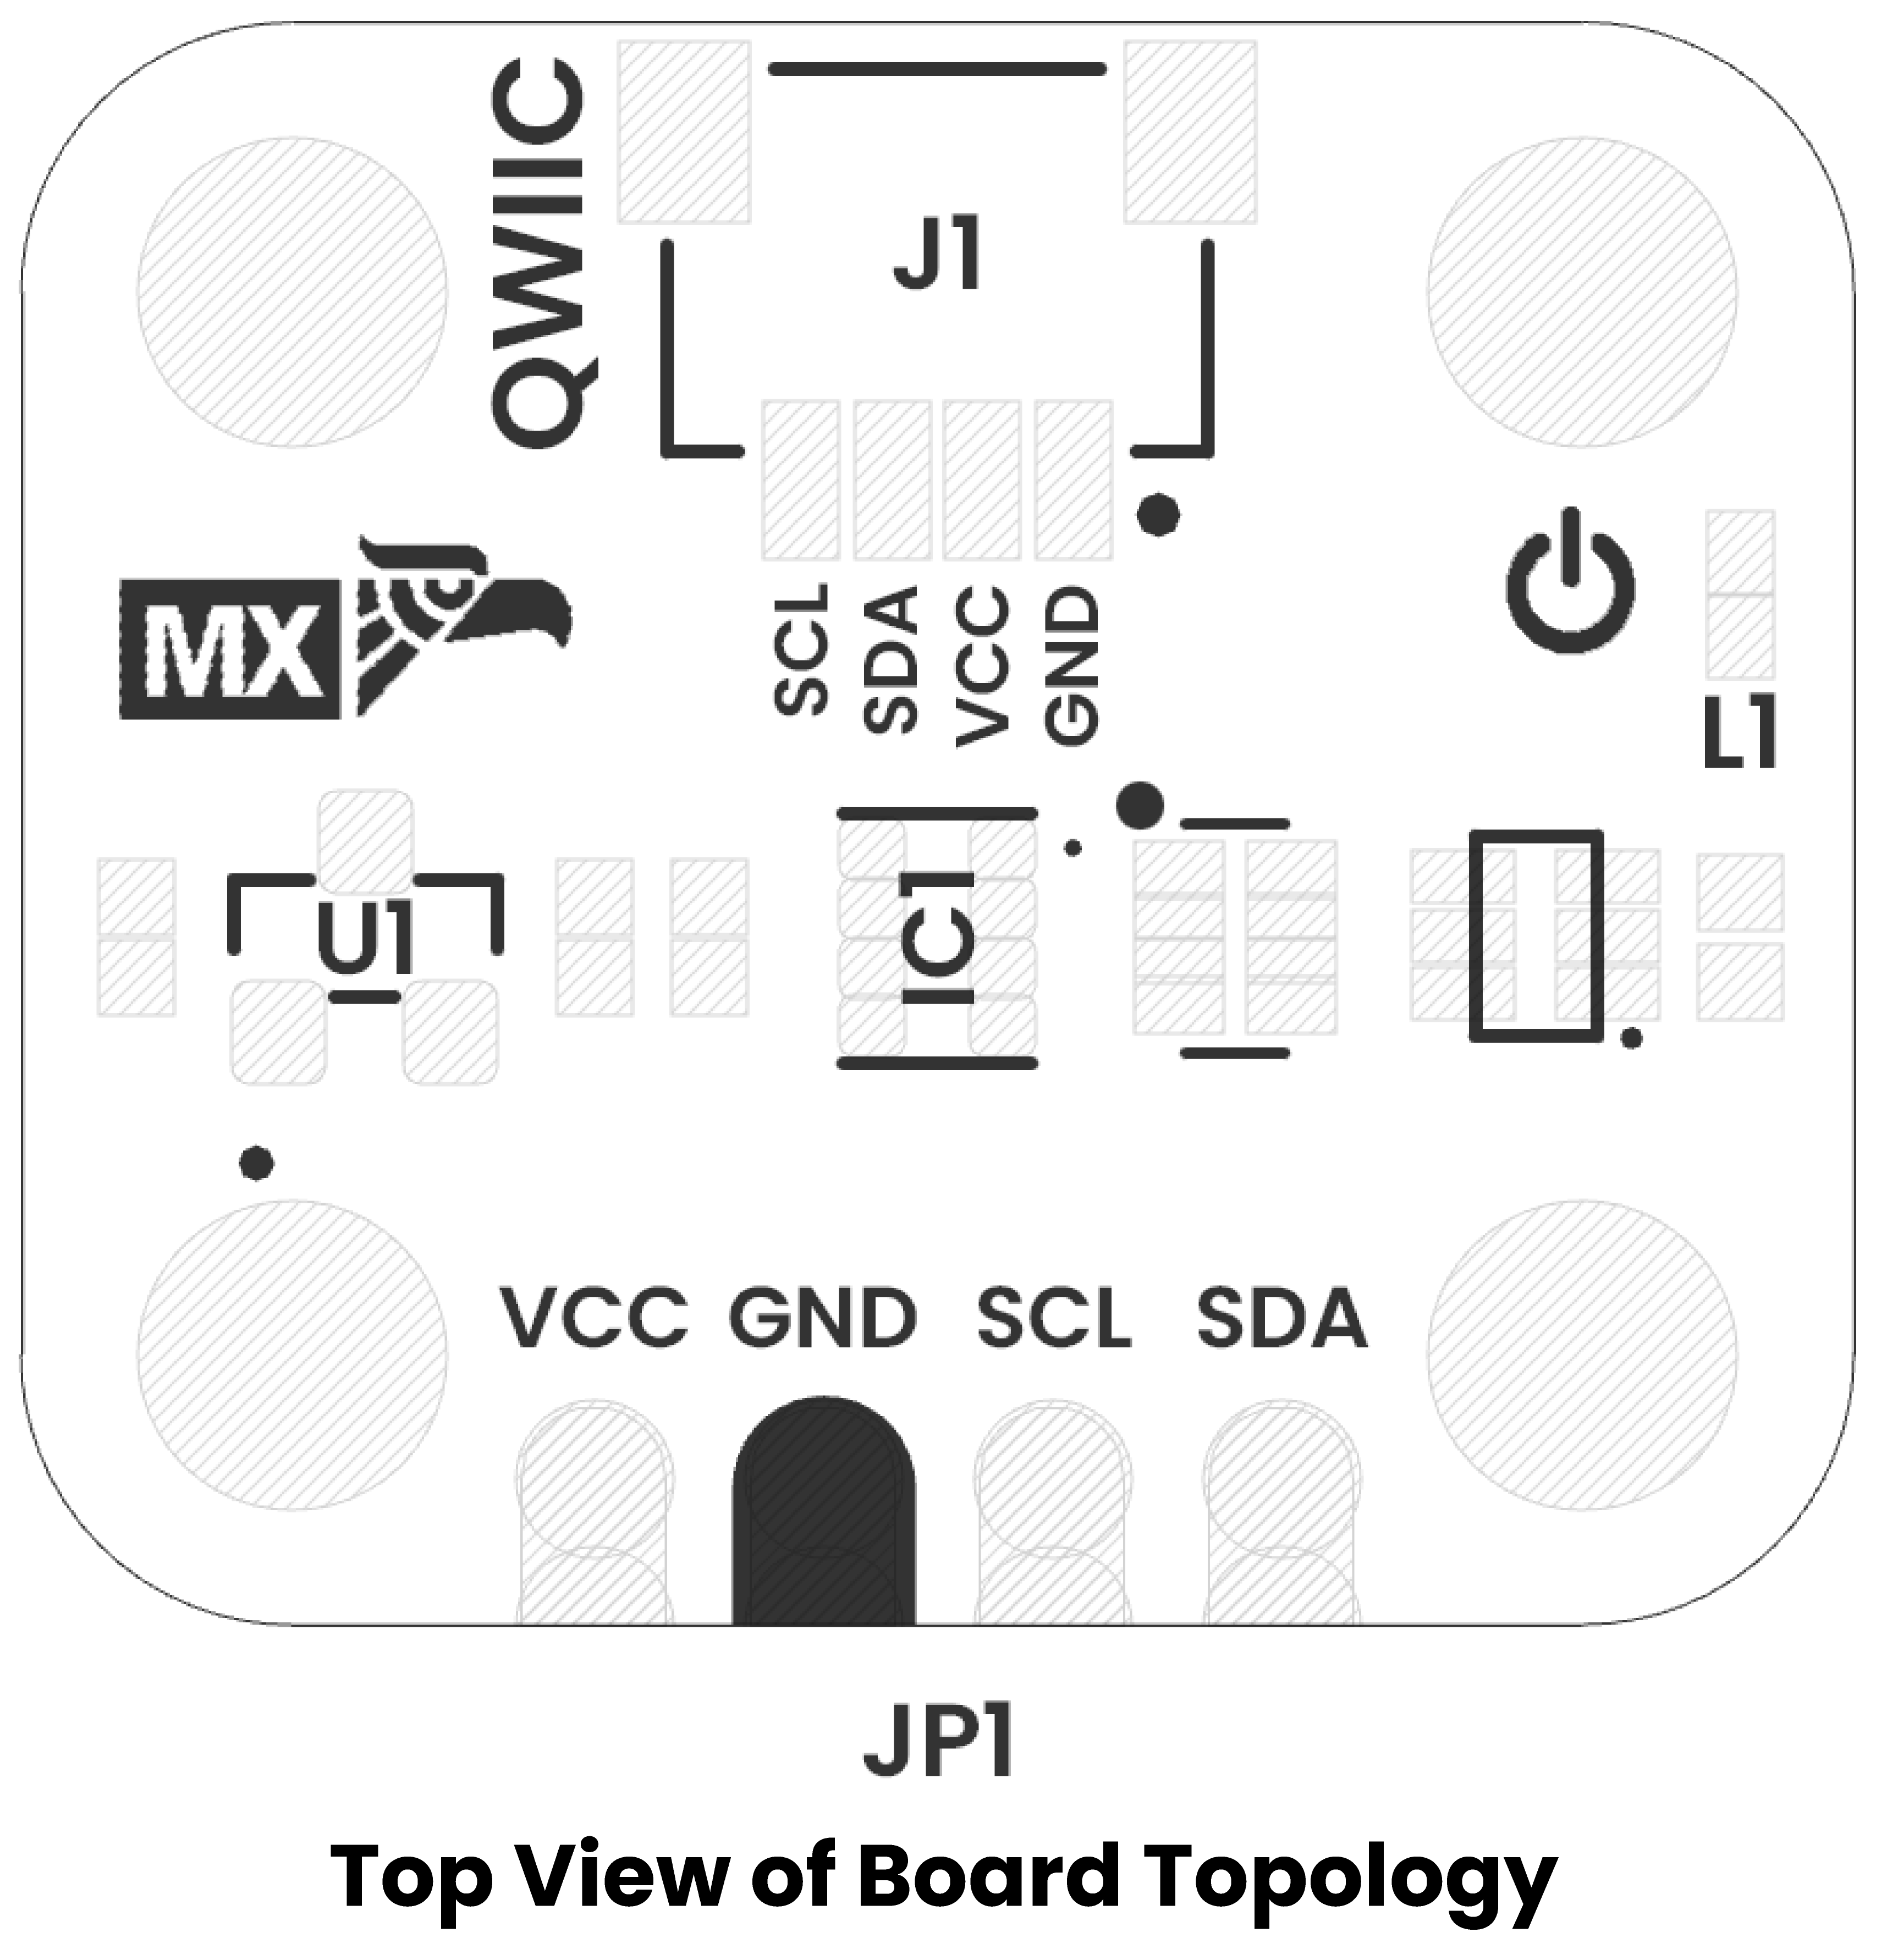
\includegraphics[width=0.7\textwidth]{es_unit_topology_v_1_0_0_icp10111_barometric_pressure_sensor.png}
\caption{Topología del Sistema}
\label{fig:es-unit-topology-v-1-0-0-icp10111-barometric-pressure-sensor-png}
\end{figure}



\subsubsection{Procesador y Memoria}


\begin{table}[H]
\centering
\small
\begin{tabular}{|l|l|l|l|}
\hline
Parámetro & Valor & Unidad & Notas \\
\hline
CPU & Dual-core Xtensa LX6 & 240 MHz & RISC de 32-bit \\
Memoria Flash & 4 MB & MB & SPI Flash externa \\
SRAM & 520 KB & KB & SRAM interna \\
Memoria RTC & 16 KB & KB & Ultra Bajo Consumo \\
\hline
\end{tabular}
\caption{Especificaciones técnicas}
\end{table}


\subsubsection{Especificaciones de Alimentación}


\begin{table}[H]
\centering
\small
\begin{tabular}{|l|l|l|l|l|l|}
\hline
Parámetro & Mín & Típ & Máx & Unidad & Condiciones \\
\hline
Voltaje de Alimentación & 2.2 & 3.3 & 3.6 & V & Operación Normal \\
Corriente Activa & - & 160 & 260 & mA & Wi-Fi Tx @ 19.5dBm \\
Corriente en Reposo & - & 5 & 10 & µA & Modo Sleep Profundo \\
Corriente Standby & - & 240 & 350 & µA & Modo Light Sleep \\
\hline
\end{tabular}
\caption{Especificaciones técnicas}
\end{table}


\subsubsection{Capacidades Inalámbricas}

\paragraph{Especificaciones Wi-Fi}
\begin{itemize}
\item \textbf{Estándares}: 802.11 b/g/n (2.4 GHz)
\item \textbf{Velocidad de Datos}: Hasta 150 Mbps
\item \textbf{Potencia de Salida}: +19.5 dBm máx
\item \textbf{Antena}: Antena PCB integrada
\end{itemize}

\paragraph{Especificaciones Bluetooth}
\begin{itemize}
\item \textbf{Versión}: Bluetooth v4.2 BR/EDR y BLE
\item \textbf{Potencia de Salida}: +9 dBm máx
\item \textbf{Alcance}: Hasta 100m (campo abierto)
\end{itemize}

\subsection{Configuración GPIO}


\begin{figure}[H]
\centering
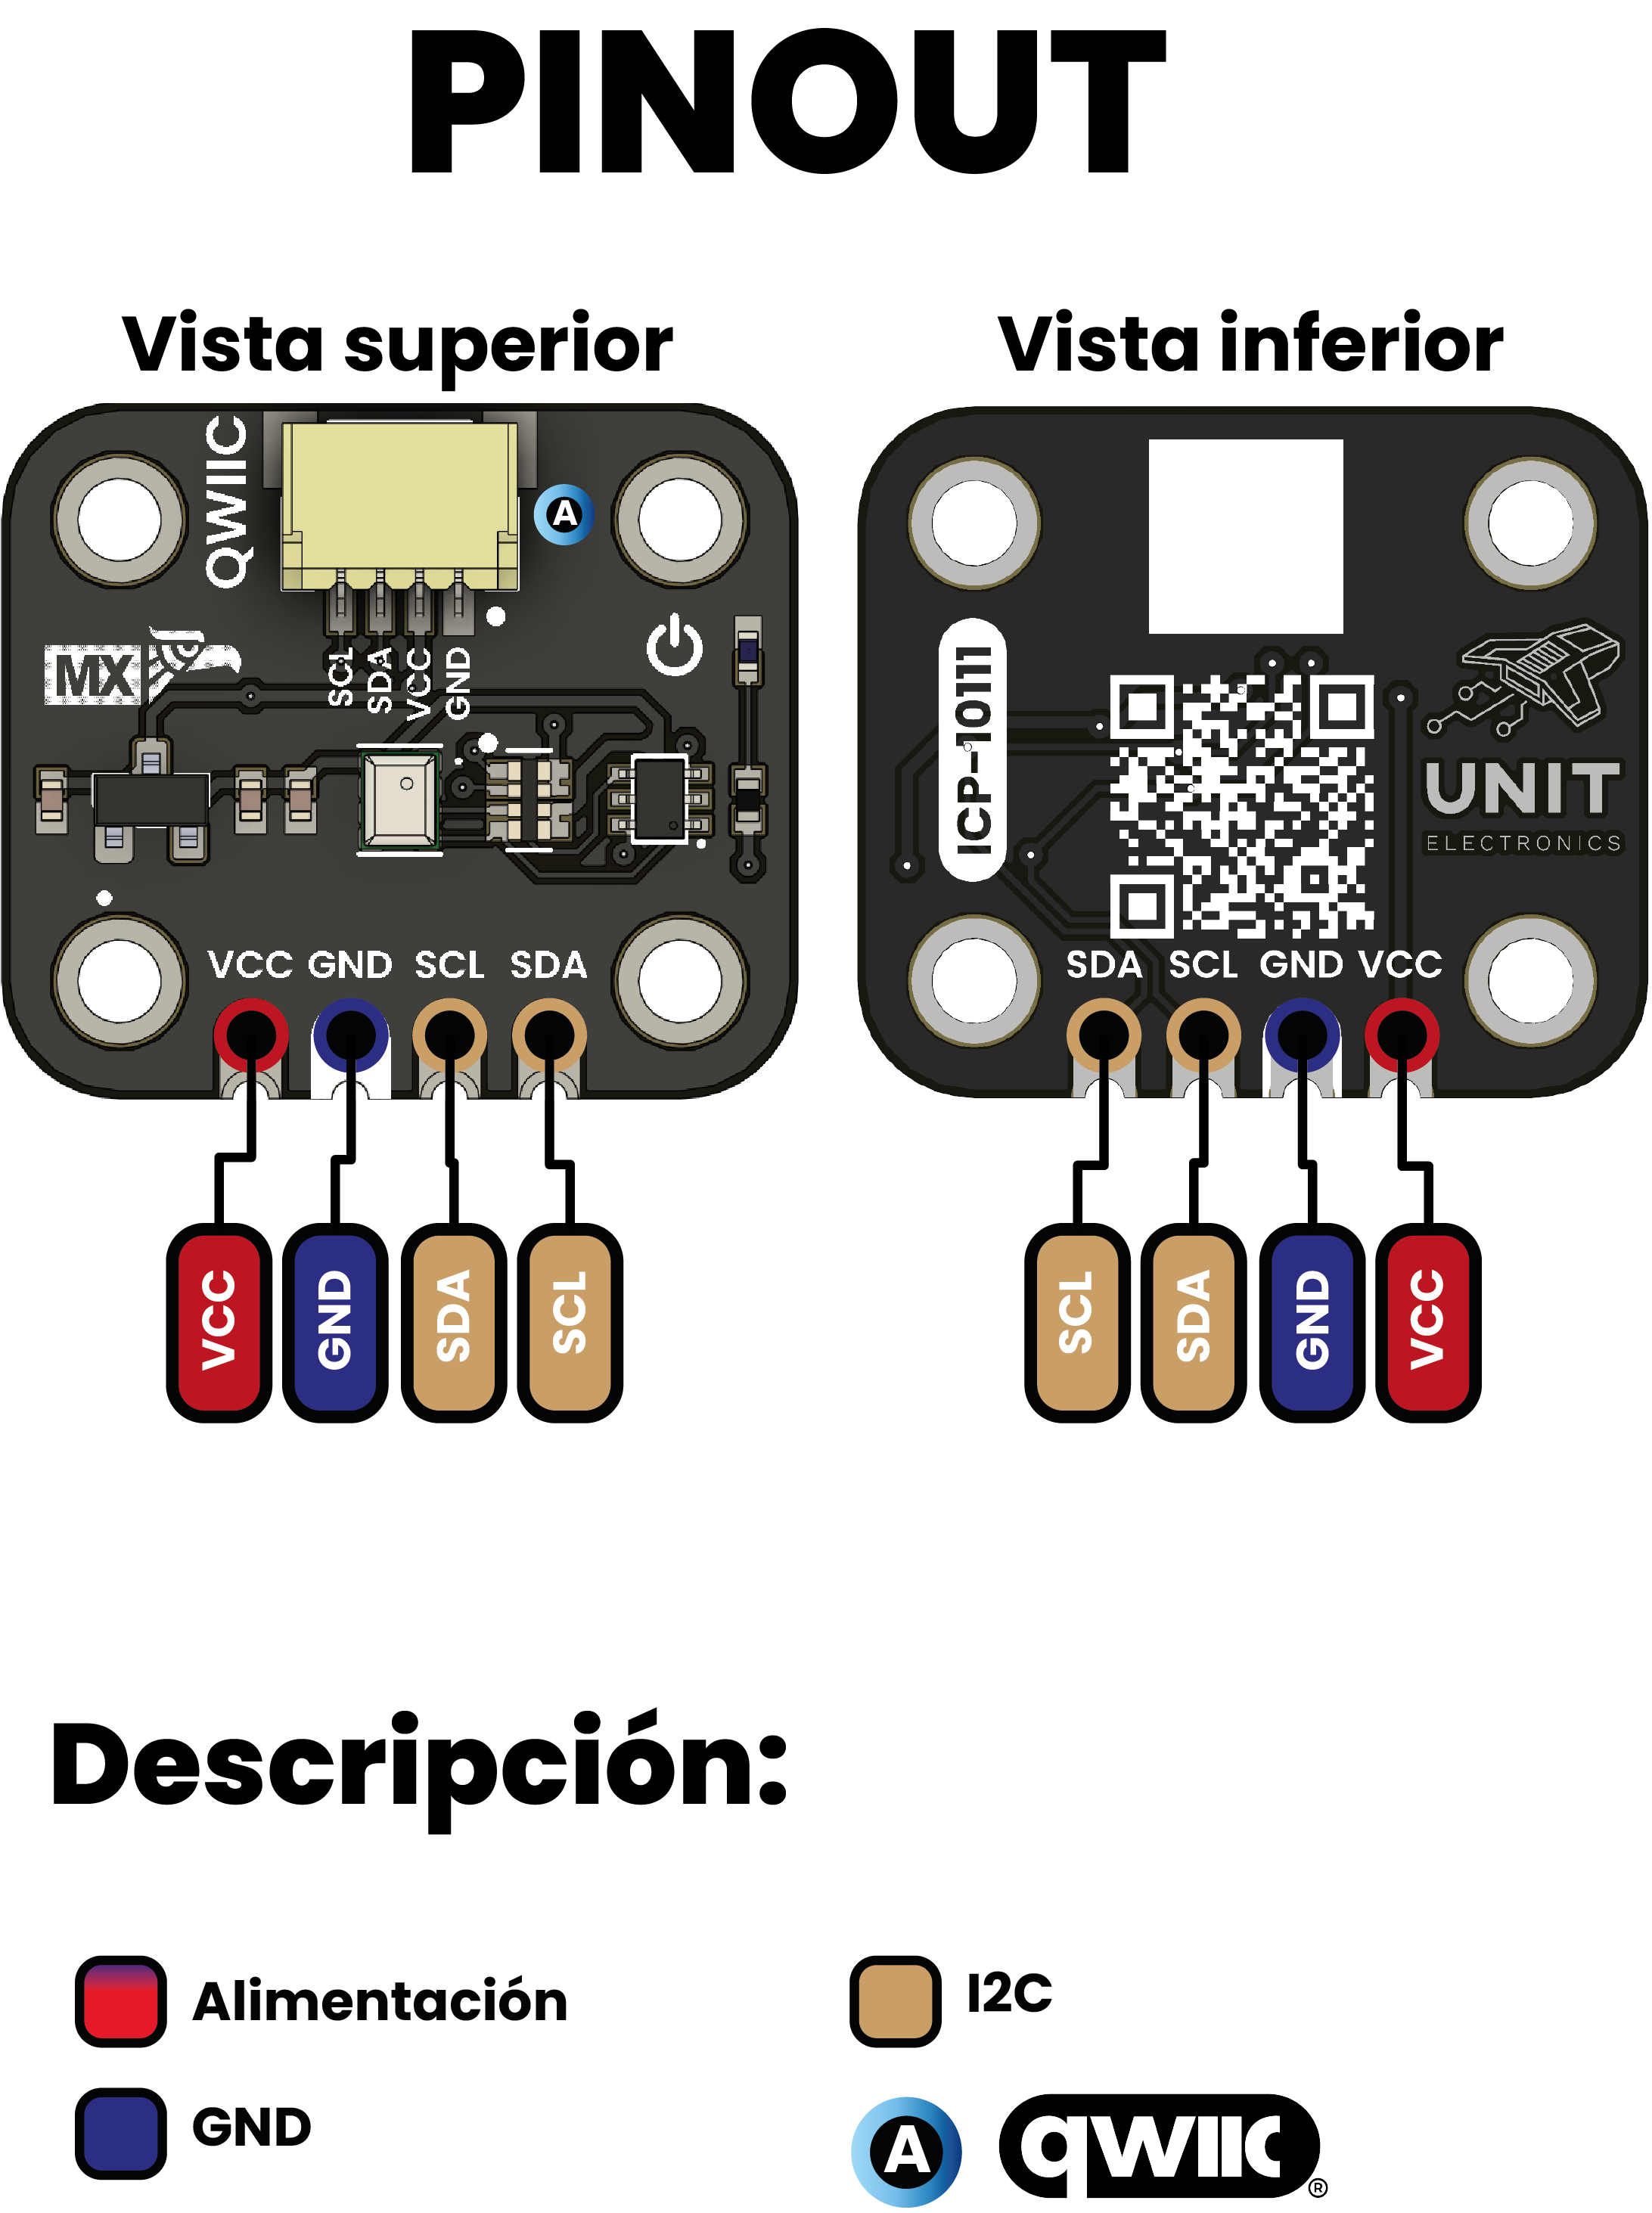
\includegraphics[width=0.9\textwidth]{es_unit_pinout_v_0_0_1_ue0094_icp10111_barometric_pressure_sensor_es.png}
\caption{Diagrama de Pines}
\label{fig:es-unit-pinout-v-0-0-1-ue0094-icp10111-barometric-pressure-sensor-es-png}
\end{figure}



\subsubsection{Pines Disponibles}


\begin{table}[H]
\centering
\small
\begin{tabular}{|l|l|l|l|l|}
\hline
Pin & Función & Voltaje & Corriente & Características Especiales \\
\hline
GPIO0 & E/S Digital & 3.3V & 40 mA & Control de arranque \\
GPIO1 & UART0_TXD & 3.3V & 40 mA & Salida debug por defecto \\
GPIO2 & E/S Digital & 3.3V & 40 mA & Control de LED \\
GPIO3 & UART0_RXD & 3.3V & - & Entrada debug por defecto \\
GPIO4-5 & E/S Digital & 3.3V & 40 mA & Propósito general \\
\hline
\end{tabular}
\caption{Especificaciones técnicas}
\end{table}


\subsubsection{Capacidades ADC}

El módulo incluye un ADC SAR de 12-bit con las siguientes características:

\begin{itemize}
\item \textbf{Resolución}: 12-bit (4096 niveles)
\item \textbf{Rango de Entrada}: 0 - 3.3V
\item \textbf{Canales}: 8 canales disponibles
\item \textbf{Velocidad de Muestreo}: Hasta 2 Msps
\end{itemize}

\subsection{Interfaces de Comunicación}

\subsubsection{UART}
\begin{itemize}
\item \textbf{Canales}: 3 controladores UART por hardware
\item \textbf{Velocidad}: Hasta 5 Mbps
\item \textbf{Características}: Control de flujo por hardware, soporte DMA
\end{itemize}

\subsubsection{SPI}
\begin{itemize}
\item \textbf{Canales}: 4 controladores SPI
\item \textbf{Velocidad}: Hasta 80 MHz
\item \textbf{Modos}: Operación Maestro/Esclavo
\item \textbf{Características}: Soporte DMA, mapeo flexible de pines
\end{itemize}

\subsubsection{I2C}
\begin{itemize}
\item \textbf{Canales}: 2 controladores I2C
\item \textbf{Velocidad}: Estándar (100 kHz), Rápido (400 kHz), Rápido+ (1 MHz)
\item \textbf{Características}: Soporte multi-maestro, direccionamiento 7/10-bit
\end{itemize}

\subsection{Características Físicas}


\begin{figure}[H]
\centering
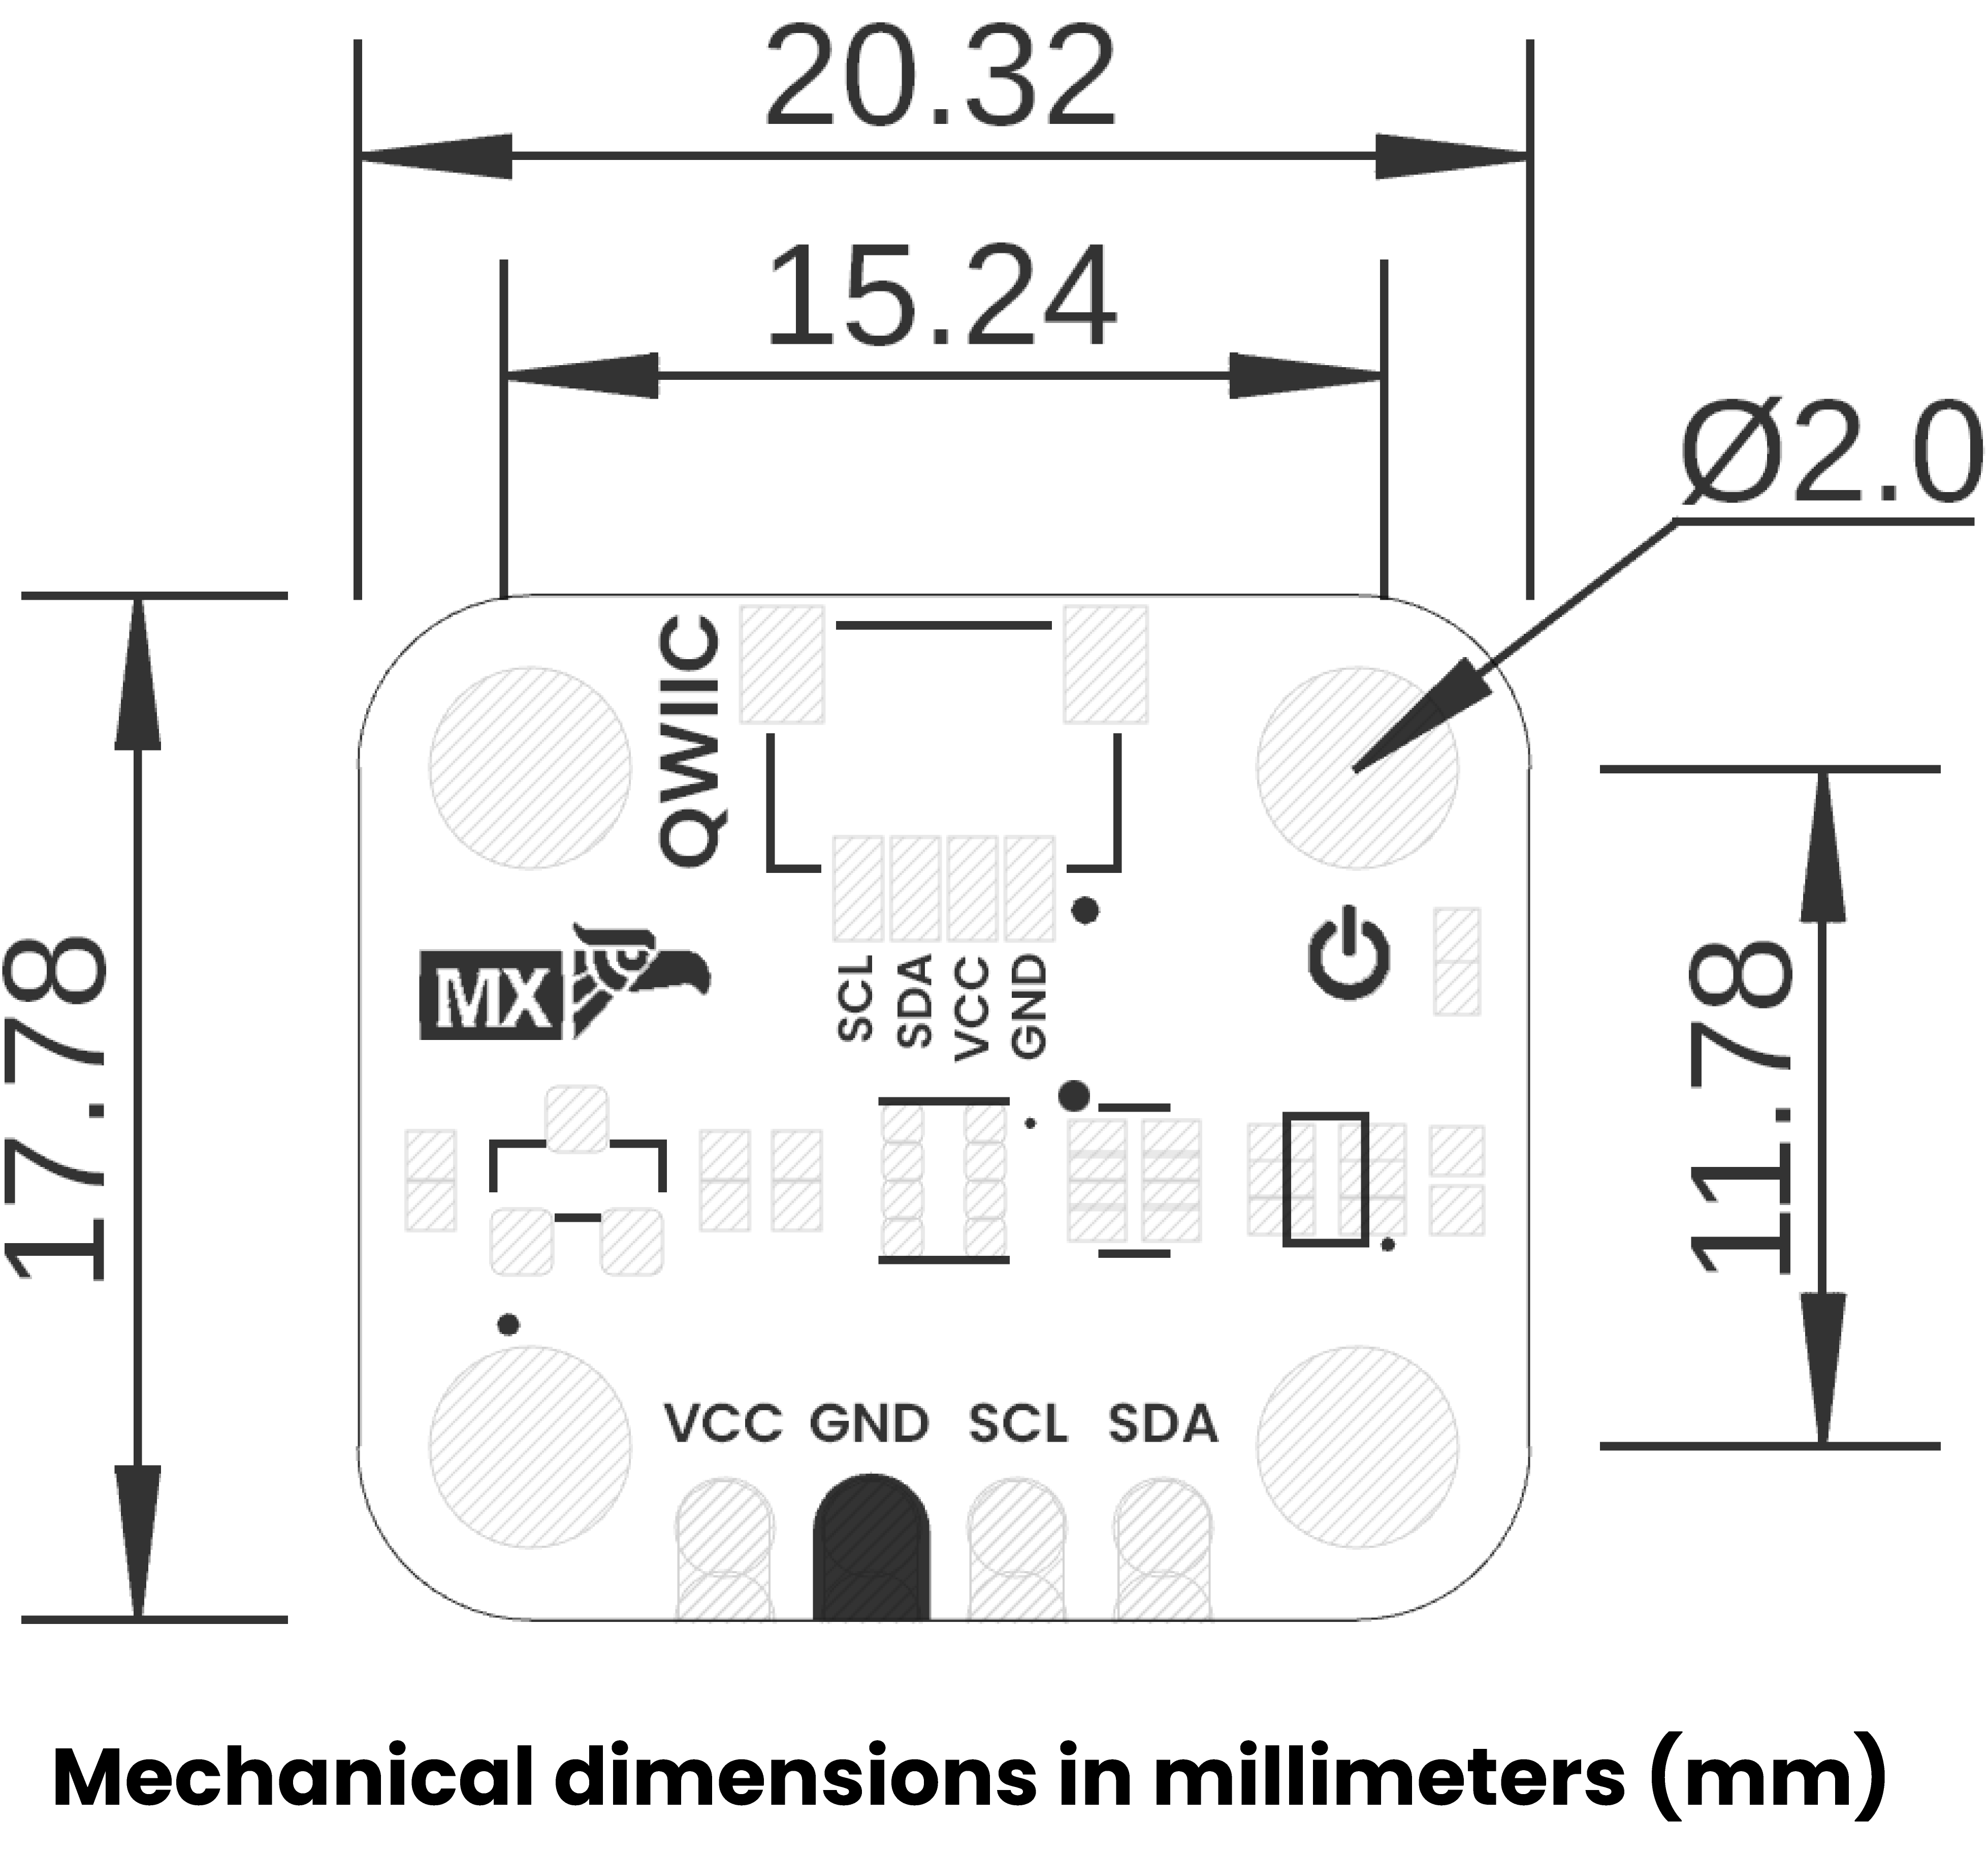
\includegraphics[width=0.6\textwidth]{es_unit_dimension_v_1_0_0_icp10111_barometric_pressure_sensor.png}
\caption{Dimensiones Físicas}
\label{fig:es-unit-dimension-v-1-0-0-icp10111-barometric-pressure-sensor-png}
\end{figure}




\begin{figure}[H]
\centering
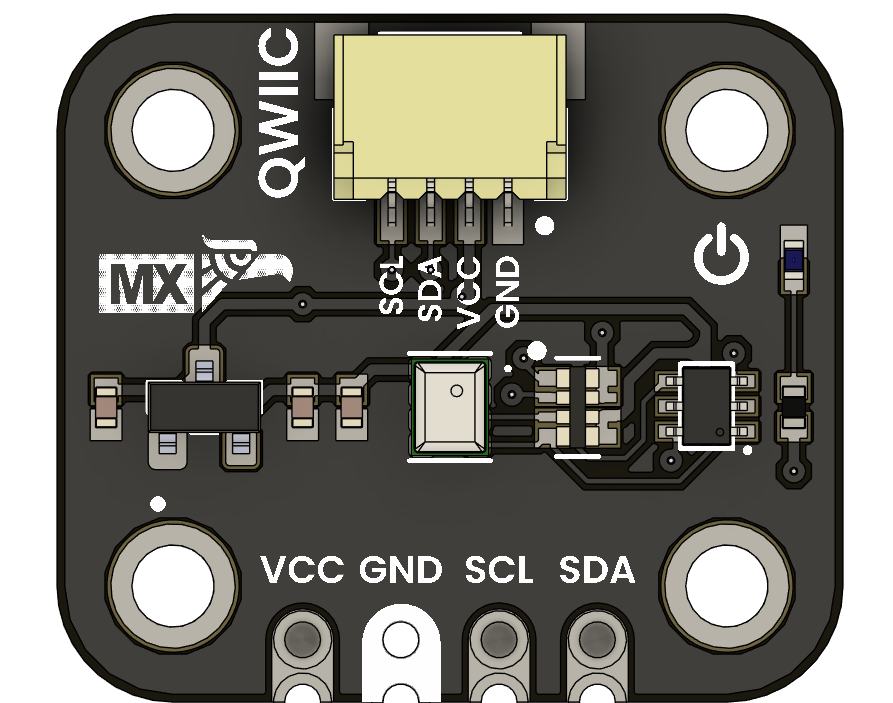
\includegraphics[width=0.7\textwidth]{es_unit_top_v_1_0_0_icp10111_barometric_pressure_sensor.png}
\caption{Vista Superior}
\label{fig:es-unit-top-v-1-0-0-icp10111-barometric-pressure-sensor-png}
\end{figure}




\begin{figure}[H]
\centering
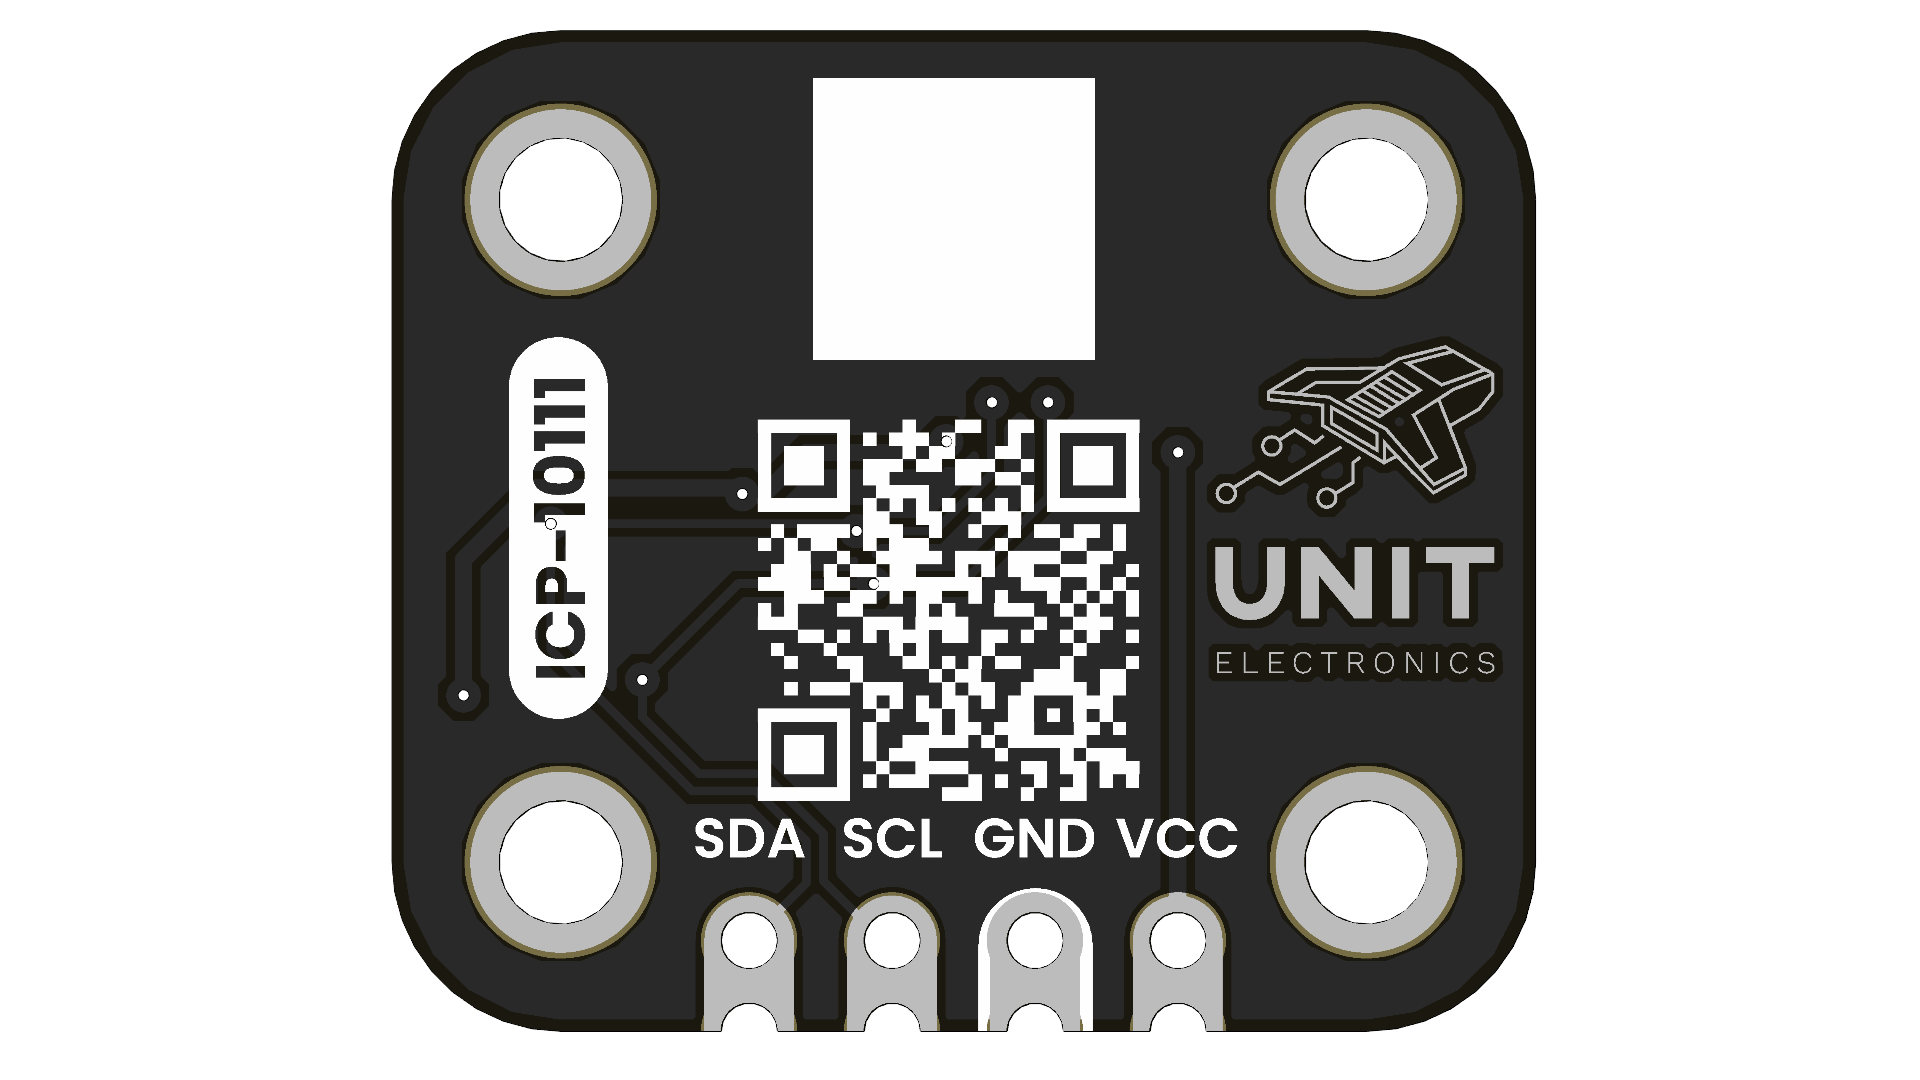
\includegraphics[width=0.7\textwidth]{es_unit_btm_v_1_0_0_icp10111_barometric_pressure_sensor.png}
\caption{Vista Inferior}
\label{fig:es-unit-btm-v-1-0-0-icp10111-barometric-pressure-sensor-png}
\end{figure}



\subsubsection{Información del Encapsulado}


\begin{table}[H]
\centering
\small
\begin{tabular}{|c|c|c|}
\hline
Parámetro & Valor & Unidad \\
\hline
Tipo de Encapsulado & QFN-48 & - \\
Dimensiones & 6 x 6 x 0.9 & mm \\
Separación de Pines & 0.4 & mm \\
Peso & 0.5 & g \\
\hline
\end{tabular}
\caption{Especificaciones técnicas}
\end{table}


\subsubsection{Especificaciones Ambientales}


\begin{table}[H]
\centering
\small
\begin{tabular}{|l|l|l|l|l|}
\hline
Parámetro & Mín & Máx & Unidad & Condiciones \\
\hline
Temperatura de Operación & -40 & +85 & °C & Grado comercial \\
Temperatura de Almacenamiento & -55 & +125 & °C & - \\
Humedad & 10 & 95 & %HR & Sin condensación \\
\hline
\end{tabular}
\caption{Especificaciones técnicas}
\end{table}


\subsection{Soporte de Software}

\subsubsection{Entorno de Desarrollo}
\begin{itemize}
\item \textbf{Arduino IDE}: Soporte completo con núcleo ESP32
\item \textbf{ESP-IDF}: Framework nativo de Espressif
\item \textbf{PlatformIO}: Soporte IDE multiplataforma
\item \textbf{MicroPython}: Soporte Python para desarrollo rápido
\end{itemize}

\subsubsection{Librerías Principales}
\begin{itemize}
\item Conectividad WiFi & Bluetooth
\item Sistema operativo en tiempo real FreeRTOS
\item Capa de abstracción de hardware (HAL)
\item Soporte de actualización por aire (OTA)
\end{itemize}

\subsection{Aplicaciones}

El módulo DevLab es ideal para:

\begin{enumerate}
\item \textbf{Sensores y Actuadores IoT}
\end{enumerate}
\begin{itemize}
\item Monitoreo ambiental
\item Dispositivos domóticos
\item Automatización industrial
\end{itemize}

\begin{enumerate}
\item \textbf{Prototipado y Desarrollo}
\end{enumerate}
\begin{itemize}
\item Pruebas de concepto rápidas
\item Proyectos educativos
\item Aplicaciones de investigación
\end{itemize}

\begin{enumerate}
\item \textbf{Productos Comerciales}
\end{enumerate}
\begin{itemize}
\item Electrodomésticos inteligentes
\item Dispositivos vestibles
\item Iluminación conectada
\end{itemize}

\subsection{Seguridad y Cumplimiento}

\subsubsection{Certificaciones}
\begin{itemize}
\item \textbf{FCC}: Parte 15.247 (USA)
\item \textbf{CE}: EN 300 328, EN 301 489 (Europa)
\item \textbf{IC}: RSS-210 (Canadá)
\end{itemize}

\subsubsection{Características de Seguridad}
\begin{itemize}
\item \textbf{Protección ESD}: ±2kV HBM en todos los pines
\item \textbf{Inmunidad Latch-up}: ±100mA
\item \textbf{Protección Térmica}: Apagado térmico automático
\end{itemize}

\subsection{Información de Pedidos}


\begin{table}[H]
\centering
\small
\begin{tabular}{|l|l|l|l|}
\hline
Número de Parte & Descripción & Empaque & MOQ \\
\hline
DEVLAB-001 & Módulo Estándar & Bandeja & 100 \\
DEVLAB-001R & Compatible RoHS & Tape & Reel & 1000 \\
DEVLAB-DEV & Kit de Desarrollo & Caja Individual & 1 \\
\hline
\end{tabular}
\caption{Especificaciones técnicas}
\end{table}


\subsection{Historial de Revisiones}


\begin{table}[H]
\centering
\small
\begin{tabular}{|c|c|c|}
\hline
Versión & Fecha & Cambios \\
\hline
1.0 & 2025-07-18 & Lanzamiento inicial \\
\hline
\end{tabular}
\caption{Especificaciones técnicas}
\end{table}


\subsection{Esquemáticos}


\begin{figure}[H]
\centering
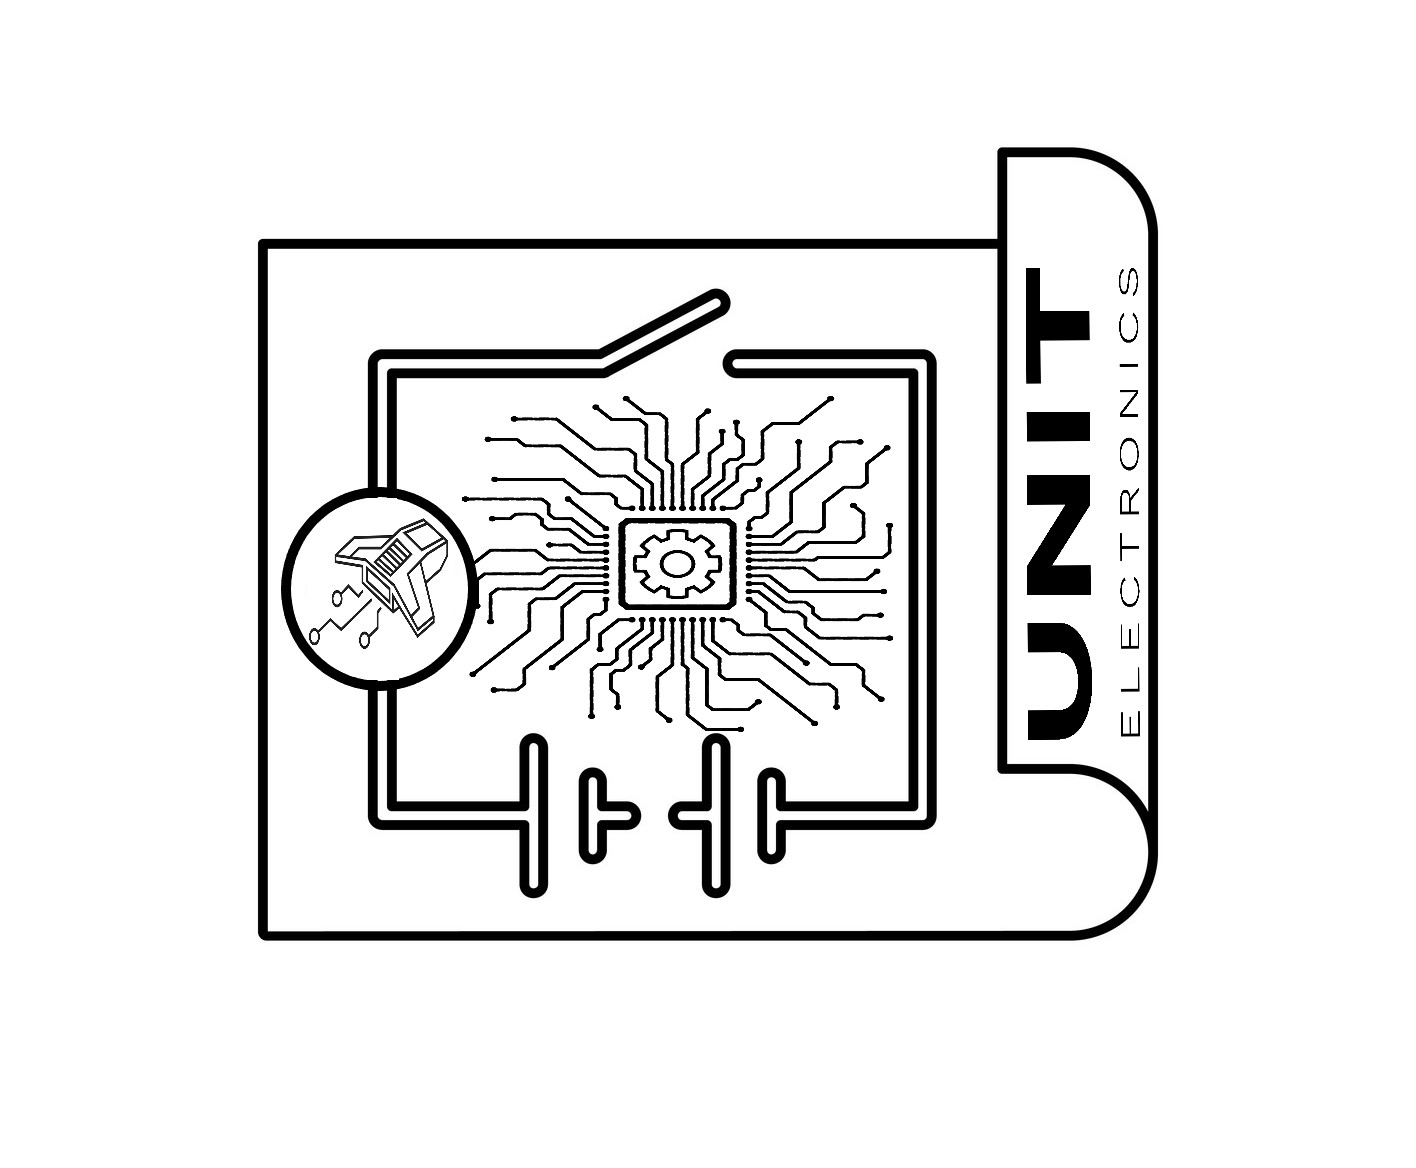
\includegraphics[width=\textwidth]{es_Schematics_icon.jpg}
\caption{Esquemático del Circuito}
\label{fig:es-Schematics-icon-jpg}
\end{figure}



---

\textit{Para soporte técnico e información adicional, visita nuestro sitio web o contacta a nuestro equipo de ingeniería.}


\end{document}
